The models the app developed in this work uses are based on chapters 19-21 of the book
"Networks Crowds and Markets" Easley and Kleinberg \cite{networks}.

\section{Simplest model}
The first model proposed by Easley and Kleinberg \cite{networks} uses a very simplistic
representation of networks. The network is represented as a tree with each layer representing
the nodes who come into contact with infected nodes form the previous cycle. The root
of the tree is the first person to contract the disease in the social network. During the
first cycle the $k$ nodes at a depth of 1 may or may not get infected with the disease based
on the infectiousness of the disease. During the second cycle each of these $k$ nodes
now comes into contact with $k$ other nodes at a depth of 2. This means during the second
cycle $k \cdot k = k^2$ people are potentially at risk of infection. During each cycle the
amount of people that come into contact with the disease increases by a factor of $k$ for
a total of $k^{cycle}$ that potentially come into contact with the disease during each cycle.
Figure \ref{fig:tree_network} shows a possible network structure.

\begin{figure}
    \centering
    \includegraphics[width=0.5\linewidth]{images/tree_network.png}
    \caption{Tree representation of a network showing the spread of a disease (source: \cite{networks})}
    \label{fig:tree_network}
\end{figure}

The book \cite{networks} also explains the concept of the reproductive number $R_0$ in
relation to this network. $R_0$ is the expected number of new cases of the disease
caused by a single infected individual. In the case of the tree network this means 
$R_0 = pk$ with $p$ being the infectiousness of the disease. If $R_0 > 1$ the amount
of cases will increase over time because each person infects more than one other person
on average. Thus there is a possibility that the disease will never
die out. If $R_0 < 1$ the amount of cases is decreasing on average each person infects less
than one other person which leads to the disease dying out in a finite number of cycles.
With this knowledge the importance of $R_0$ in fighting an epidemic is clear. To prevent
or stop a epidemic the $R_0$ factor of a disease has to be below 0.

\subsection{Limitations}
This model has several limitations. It assumes each person has contact to the same amount of
people which is never the case in real social networks. There are always people who come into
contact with more people than others. Also each person can only infect others during the
first cycle after they got infected. It does not allow for a person to infect others during
multiple cycles for longer lasting diseases. Further it is not possible for a person
to get infected a second time as there are no loops withing the tree.

\section{SIR Model}
The SIR Model is a more advanced model that allows modeling of most social network structures
by generalizing the contact structure. Easley and Kleinberg \cite{networks} define three 
stages each node can have:
\begin{itemize}
    \item \textbf{S}usceptible: Node is not yet infected but susceptible to infection from its neighbors
    \item \textbf{I}nfectious: Node has caught the disease and has a probability to infect its neighbors
    \item \textbf{R}emoved: The node went through the full infection period and is removed from consideration for future cycles
\end{itemize}
The SIR Model uses a directed graph do indicate which nodes are neighbors and thus susceptible 
to infecting each other. The resulting graph does not have to be anti symmetric it may also contain
undirected edges. 

In addition to the network the SIR Model uses two additional quantities to control the 
epidemic: $p$ the probability an infected node infects a susceptible node and $t_I$ the length
of the infection period.

Initially some nodes are in the $I$ state while all others are in the $S$ state. After
each cycle all neighbors of the nodes in the $I$ state are infected with a probability of $p$.
After $t_I$ steps a node is removed from the $I$ state and can no longer infect others or be
infected by others.

\subsection{Reproductive Number}
For these more complex networks calculating the reproductive number $R_0$ is not as trivial
as for a tree based network. The book contains an example for a network shown in figure \ref{fig:narrow_network}
in which even highly contagious diseases will die out.

\begin{figure}
    \centering
    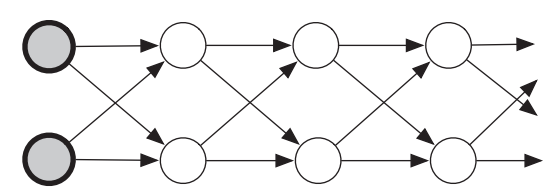
\includegraphics[width=0.5\linewidth]{images/narrow_network.png}
    \caption{A network where the disease must pass through a narrow structure of nodes. (source: \cite{networks})}
    \label{fig:narrow_network}
\end{figure}

Let $d$ be a disease with a high contagiousness of $p=0.8$ and infection period $t_I=1$. 
Using the assumptions made for calculating $R_0$ in the tree network this would result 
in $R_0 = 2 \cdot 0.8 = 1.6$ which indicates that the disease is relatively likely 
to never die out. Due to the structure of the network however, the disease is going to 
die out relatively quickly. The chance of the disease not spreading during a cycle is
$0.2^4=0.0016$ thus the disease will on average die out after $\frac{1}{0.0016}=625$ cycles.
This shows that in more complex networks the structure of the network also plays a big role
in the progression of the epidemic. It is not possible to calculate $R_0$ using just the
characteristics of the disease, the network structure also needs to be taken into account.
Knowing this it is impossible to accuarately calculate $R_0$ in a highly complex network.
It is however possible to observe the $R_0$ value during the epidemic for previous cycles.
Let $R_0^k$ be the $R_0$ value for cycle $k$ and $I_k$ the amount of infected nodes in cycle $k$.
Then $R_0^k = \frac{I_k}{I_{k-1}}$, with this the evolution of the $R_0$ value can be 
observed making it possible to estimate $R_0$ for future cycles and helping to understand
whether the disease is currently dying out ($R_0<0$) or not ($R_0>1$). A simulation can also
help to understand how the $R_0$ value of diseases will behave for a disease with certain 
quantities in a complex network.

\subsection{Limitations}
There are still some limitations to the SIR Model. Each person can only catch the disease at
most once and the model does not allow for simulating multiple diseases at the same time.
However the model allows most social networks to be represented, making it realtively easy
to extend this network to include more complex diseases with different levels of contagiousness
depending on the time a node has been infected or a non constant infection period.

\section{SIS Model}
The SIS Model is an extension to the SIR Model which also allows nodes to be reinfected multiple
times. The \textbf{R}emoved state is exchanged with the \textbf{S}usceptible state, so nodes
that are removed from the \textbf{I}nfected state are placed back in the \textbf{S}usceptible state.
With this change it is possible for diseases to last an inifinite time in a SIS Model in contrast
to an SIR Model where every simulation will end after a finite amount of steps after the 
disease burned through all nodes. The only way for the simulation in a SIS Model to end is
if all infected nodes fail to transmit the disease to any of their neighbors $t_I$ times.

\section{Custom Model}
\subsection{Parameters}
The model used by the developed app is a further extension to the SIR and SIS Models. It 
combines the SIR and SIS Model by having nodes that finish the infection period move either
into the \textbf{R}emoved or \textbf{S}usceptible state depending on a quantity $f$. Each
disease has a fatality rate $f$ which determines whether a node is moved into the 
\textbf{R}emoved state and considered deceased or moved back into the \textbf{S}usceptible
state if it survived the infection. The \textbf{S}usceptible state will be split into two
substates: nodes that never were infected before nad nodes that were put back into it after
being infected at least once. This allows for different infectiousness values $p_I$ for the
first infection of a node and $p_r$ for reinfections. 

The $t_I$ parameter will be split into two new parameters $t_{min}$ the minimum time an infection takes
before the node can be cured and $t_\rho$ the probability a node is cured from its infection
after the minimum time $t_{min}$ has elapsed. This results in four states so far:

\begin{itemize}
    \item Healthy: Susceptible nodes that were never infected before. They are at risk of being
    infected by their neighbors with a probability of $p_I$
    \item Infected: Nodes that are currently infected. The infection duration is least $t_{min}$ cycles and
    the exact duration is determiend by the probability $t_\rho$. After the infection ended the
    node is moved into the cured state with probability $1-f$ or into the deceased state with
    probability $f$.
    \item Cured: Nodes that were infected but survived. They are at risk of being
    infected by their neighbors with a probability of $p_r$ 
    \item Deceased: Nodes that died from the infection. They are not considered in future cycles
    and can not infect others anymore.
\end{itemize}

The infectiousness of a disease usually changes over the duration of the infections. In most
cases an infected person is most likely to infect other during the first few days of contracting
a disease. This should also be represented in the custom model. Thus the $p_I$ and $p_r$ values
need to change with the time a node has been infected $t_c$. These time dependant probabilities
will be called $p_I^t$ and $p_r^t$. A healthy node now has a probability of $p_I^t$ to
be infected by another node that is infected since $t$ cycles. Analogue a cured node 
now has a probability of $p_r^t$.

Another part of epidemics that is not represented in the SIR or SIS Model is vaccines.
During the course of an epidemic vaccines may be used which decrease the fatality rate
for infected persons and decrease the likelyhood for vaccinated person to be infected with
the disease. To incorporate this in the custom model two new states for nodes are added:
\begin{itemize}
    \item Vaccinated: Nodes that are vaccinated and now have a probability of getting infected
    of $p_v^t$ and a fatality rate of $f_v$.
    \item Unvaccinated: Nodes that are not vaccinated and use the above mentioned probabilities
    $p_I^t$/$p_r^t$ and $f$.
\end{itemize}
These two new states are not exclusive with the previous four states. Each node simultaneously
has one of the two states, vaccinated or unvaccinated, and one of the previous four states 
healthy, cured, infected or deceased.

\subsection{Network model}
The network model is very similar to the one used by the SIR and SIS Model. However it does
not allow for directed connections as there are very limited uses for those connections. 
Almost every human contact is bidirectional if for example one person gets close enough to
another person to contract an air transmitted disease this transmission can always happen
in both directions.

The network model used in this custom model organizes the nodes of one social circle in groups
to more clearly organize the network for more visual clarity. Each group can be 
considered a small-world %TODO ref
contact network were the nodes in each group are a localized part
of the network that is highly connected with fewer connections to other groups.

\section{Characteristics of epidemics}
\subsection{Oscillating diseases}
As explained by Easley and Kleinberg \cite{networks} diseases with certain characteristics
can cause an oscillating amount of infection. Consider a network with multiple highly
connected groups that have only have a few connections between the groups. If a disease
with a very high infection probability $p\geq0.9$, a period of immunity $i > 0$ and a
fatality rate close to zero breaks out in such a network, the infection amount will osciallate.
An example how the number of infections could evolve over time can be seen in figure 
\ref{fig:oscillation}.
\begin{figure}
    \centering
    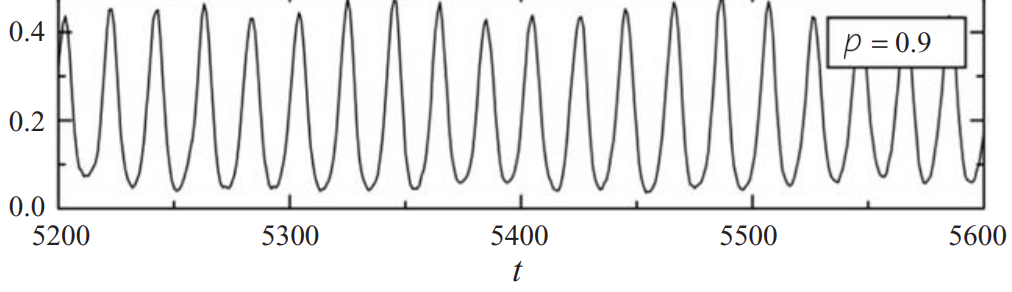
\includegraphics[width=0.5\linewidth]{images/oscillation.png}
    \caption{Amount of infections over time in a network of highly connected 
    groups. The disease has a high infection rate and low fatality. (source: \cite{networks})}
    \label{fig:oscillation}
\end{figure}

This happens because due to the high infectiousness of the disease almost all nodes of 
a group that has at least one infected node will be infected within a few cycles. Because
almost all nodes are infected after only a few cycles there are only a few new infections 
in the next cycles because of the sparse set of available healthy nodes. If the initial
wave started at cycle $c$ then at cycle $c' = c + t_i + i$ the nodes of the first wave 
are susceptible to infection again. Thus the amount of possible targets for new infections
increases drastically which causes the new infections to also rise again. This results in 
the oscillation of the amount of new infections.

Such a scenario can be modeled with the created tool. The network consists of 5 groups 
each having a lot of inner group connections and only a small amount of connections to the
other groups. The network contains a total of 10,000 nodes, 2,000 in each group,
its structure can be seen in figure %TODO

The disease that will be simulated in this network has a infection rate of 0.9, a fatality
rate of 0, a infection duration of 5 cycles and a immunity period of 3 cycles. For simplicity
the reinfection rate is the same as the initial infection rate and no vaccinations are used.

Initially 2 random nodes will be infected with the disease. Figure %TODO
shows the state of the network after 0, 3, 7 and 10 cycles. Currently the occilations
of the different groups are not yet synchronized. But after some more cycles they start
to synchronize as seen in figure %TODO
which shows the network after %TODO cycles
The amount of infections over time can be seen in figure %TODO
which clearly shows the oscillating nature of this disease.

Now the same network is used but the infection rate of the disease is decrease to 0.2.
Because the desease is now not spreading as explosively as before it always has enough targets
to infect until the previously infected nodes become cured again. Thus the amount of new 
infections is more consistent as seen in figure %TODO

Another way to break the oscillation is to decrease the duration of the infection to 2 cycles 
and remove the immunity period. Now the infected nodes become cured so fast that there are
enough new nodes to infect for every cycle thus again resulting in a relatively consistent
amount of new infections as indicated in figure %TODO

\subsection{Epidemics without diseases}
Diseases are not the only thing that is capable of spreading through social networks. As
previously mentioned computer viruses spread in a similar pattern. However there are other
completely different things that can spread in social networks in a similar way.
Information for example can be modeled using a very similar approach to the one proposed
for diseases. Information can be passed from person to person whenever they talk to each other
be that over a long distance through things like text messages or by meeting in person.

Other things that can spread through social networks include traditions or certain habits.
Looking at the world people within each country come into contact with other people from the
same country much more frequently than with people from other countries. This means each
country can be modeled as a highly connected group of people with few connections to other
countries. This model can be used to explain how each country has its own traditions that
differ from other countries the further away they are. Traditions spread easily within 
a country but the further away a country is the less likely the tradition is to spread to it.
As there are only few connections to other countries foreign traditions which only spread there
rarely are drowned out by the explosively spreading regional traditions of the country.

These models can also be used to model genetical inheritance. As suggested by
Easley and Kleinberg \cite{networks} this can be done by connecting parents to their offspring.
Then simulations can be run to show the spreading of different genetical factors throughout
the ancestry trees. This type simulation itself offers a lot of areas that can be expanded
on to create various simulations relevant to understanding human history and origin. 
It can also be used to indicate and visualize the existance of common ancestors and 
can give an idea of how many generations it takes to reach those. One such model that deals
with genetics and common ancestors is the Wright-Fisher Model. Haller and Messer \cite{genetics}
go into more detail how this model and the genetic simulation works. Genetic simulations 
and the Wright-Fisher Model are a big research area themselfes there are various other
works that talk about those topics, explaining the mathematics behind those models, 
possible uses etc. \cite{genetics2} \cite{genetics3} \cite{genetics4}.


This shows how the use of epidemics and social networks goes way beyond just diseases and
can help us understand complex relations in various different areas of research.